\PassOptionsToPackage{unicode=true}{hyperref} % options for packages loaded elsewhere
\PassOptionsToPackage{hyphens}{url}
%
\documentclass[]{article}
\usepackage{lmodern}
\usepackage{amssymb,amsmath}
\usepackage{ifxetex,ifluatex}
\usepackage{fixltx2e} % provides \textsubscript
\ifnum 0\ifxetex 1\fi\ifluatex 1\fi=0 % if pdftex
  \usepackage[T1]{fontenc}
  \usepackage[utf8]{inputenc}
  \usepackage{textcomp} % provides euro and other symbols
\else % if luatex or xelatex
  \usepackage{unicode-math}
  \defaultfontfeatures{Ligatures=TeX,Scale=MatchLowercase}
\fi
% use upquote if available, for straight quotes in verbatim environments
\IfFileExists{upquote.sty}{\usepackage{upquote}}{}
% use microtype if available
\IfFileExists{microtype.sty}{%
\usepackage[]{microtype}
\UseMicrotypeSet[protrusion]{basicmath} % disable protrusion for tt fonts
}{}
\IfFileExists{parskip.sty}{%
\usepackage{parskip}
}{% else
\setlength{\parindent}{0pt}
\setlength{\parskip}{6pt plus 2pt minus 1pt}
}
\usepackage{hyperref}
\hypersetup{
            pdftitle={Chudi Thesis},
            pdfauthor={Chudi Gong},
            pdfborder={0 0 0},
            breaklinks=true}
\urlstyle{same}  % don't use monospace font for urls
\usepackage[margin=1in]{geometry}
\usepackage{graphicx,grffile}
\makeatletter
\def\maxwidth{\ifdim\Gin@nat@width>\linewidth\linewidth\else\Gin@nat@width\fi}
\def\maxheight{\ifdim\Gin@nat@height>\textheight\textheight\else\Gin@nat@height\fi}
\makeatother
% Scale images if necessary, so that they will not overflow the page
% margins by default, and it is still possible to overwrite the defaults
% using explicit options in \includegraphics[width, height, ...]{}
\setkeys{Gin}{width=\maxwidth,height=\maxheight,keepaspectratio}
\setlength{\emergencystretch}{3em}  % prevent overfull lines
\providecommand{\tightlist}{%
  \setlength{\itemsep}{0pt}\setlength{\parskip}{0pt}}
\setcounter{secnumdepth}{0}
% Redefines (sub)paragraphs to behave more like sections
\ifx\paragraph\undefined\else
\let\oldparagraph\paragraph
\renewcommand{\paragraph}[1]{\oldparagraph{#1}\mbox{}}
\fi
\ifx\subparagraph\undefined\else
\let\oldsubparagraph\subparagraph
\renewcommand{\subparagraph}[1]{\oldsubparagraph{#1}\mbox{}}
\fi

% set default figure placement to htbp
\makeatletter
\def\fps@figure{htbp}
\makeatother


\title{Chudi Thesis}
\author{Chudi Gong}
\date{18/06/2020}

\begin{document}
\maketitle

\hypertarget{abstract}{%
\section{1.Abstract}\label{abstract}}

\hypertarget{introduction}{%
\section{2.Introduction}\label{introduction}}

As human beings we often make statements such as `I am confident
that\ldots{}', reflecting the importance of confidence, which has wide
applications in fields such as medical diagnosis, financial choices and
eyewitness testimony etc.. Confidence can be defined as `a belief about
the validity of our own thought, knowledge or performance that relies on
a subjective feeling.' (Grimaldi, Lau, and Basso 2015). The confidence
of one decision can bear on another decision, such as when one decides
to drop a stock investment after purchasing. The formation of confidence
in human perception has been investigated extensively, with developments
of various behavioural, neural and computational models.

Traditionally, research investigating how confidence is formed with
regards to perception commonly used detection and discrimination tasks,
which are considered to represent the very basics of our perceptual
abilities. A detection task requires to identify the presence of a
stimulus (e.g.~whether a dot is present or absent) whereas a
discrimination task (sometimes labelled as categorization) requires to
distinguish a target stimulus from other distractors based on certain
features (e.g.~whether the line is tilted to the left or the right).
Although they are both perceptual tasks, evidence has suggested they can
lead to differences in objective performance (e.g. (Mack and Palmeri
2010)), which has been investigated extensively in past decades. Until
recent years, with increasing popularity in investigating confidence
formation, studies showed that detection and discrimination can also
lead to distinctive subjective judgements of performance behaviourally
((Meuwese et al. 2014)) and neuroimaging data suggested different neural
representations associated with judging confidence in these two tasks
(e.g. (Mazor, Friston, and Fleming 2020)). Models that have been put
forward to explain such differences can be broadly divided into two
camps: 1.) Confidence judgements is a higher-order process that treats
detection and discrimination distinctively due to the differences in the
control of one's internal state, such as attention; 2.) Behaviour and
neural activities differ as a response to the physical features of
detection and discrimination at the perceptual level such as amount of
sensory evidence and confidence is formed through similar process for
these two tasks.

The current project aims to explain the distinctive processes involved
in confidence formation in detection and discrimination tasks from the
perspective of Signal Detection Theory (SDT), using a new paradigm which
includes a discrimination task with the features of detection task. This
paradigm also sheds a light on our understanding of alternative models.
The following section will first review behavioural and neuroimaging
evidence showing differences in detection and discrimination tasks, then
discuss some models that have been put forward to explain such
differences and finally propose the hypothesis that distinctive patterns
arise in forming confidence in the two tasks as a result of their
different distributions of signal (target) and noise (distractor) based
on SDT.

\hypertarget{detection-vs.discrimination}{%
\subsection{2.1. Detection
vs.~Discrimination}\label{detection-vs.discrimination}}

How do we detect and/or categorise something? Does one first detect
something is there (e.g. `I saw something is there') and then further
categorize it to certain type (e.g. `The thing I saw is a car.'), or we
know what it is immediately when we see something is there (e.g. `I saw
a car there)? The level of independence of these two tasks has been the
most commonly debated discussion regarding these two tasks ((Mack and
Palmeri 2010); (Grill-Spector and Kanwisher 2005)). This is an important
consideration for wide range of research themes, as it affects the
flexibility of using these two tasks in the investigation of other
domains such as confidence formation. Researchers advocate the view that
detection and discrimination are two process happen simultaneously

On the other hand, Mack and Palmeri (2010) used a paradigm to assess the
level of dependence of detection and discrimination at the basic-level
(car vs.~boats) and superordinate level (e.g.~car vs.~people). They
found that detection and basic-level object categorisation is supported
by single mechanism as their results revealed a dependence between the
success for the detection task and the success for basic-level
categorisation task. However, the success for one to correctly
categorize a target at superordinate level is not dependent on the
success at detection, which suggests distinctive mechanisms supporting
detection and superordinate categorisation, thus again highlighting the
importance of differentiating the two for future research. Findings from
their research reflects the importance of distinguishing between
different levels of stimuli, challenging the view of one underlying
perceptual ability for, or at least strong dependence between detection
and discrimination suggested previously by Grill-Spector and Kanwisher
(2005).

Detection and discrimination tasks also differ from the perspective that
the two alternatives rely on asymmetrical sensory evidence for detection
in contrast to symmetrical evidence for discrimination. In a detection
task, virtually no sensory evidence is available for participants to
make an absence decision, a feature that essentially makes up the
definition of `absent' in such tasks, in contrast to a present decision.
On the other hand, in discrimination tasks sensory evidence is available
for both alternative choices. This results in significant differences
from the perspective of SDT (see section 2.5 for details).

\emph{However}, \emph{despite the lack of sensory evidence in absence
conditions}, \emph{it has been found that neurons encode both stimulus
absence and presence when dissociated from motor response (Merten \&
Nieder, 2014)}. \emph{In their study}, \emph{they found that prefrontal
cortex (PFC) is recruited in rhesus monkeys during stimulus present
trials as well as absence trials using single neuron recordings}.

\hypertarget{forming-confidence-in-detection-and-discrimination}{%
\subsection{2.2. Forming confidence in detection and
discrimination}\label{forming-confidence-in-detection-and-discrimination}}

The ability to have insight into the objective correctness of a response
is known as one's metacognitive sensitivity/accuracy ((Fleming et al.
2010)). Metacognitive sensitivity is measured by calculating the level
of correspondence between the Type I objective performance and Type II
subjective report. Type II report requires participants to give
confidence ratings as participants are instructed to give high
confidence ratings when they believed their choice was correct and low
confidence ratings if they are less certain. However, it might come as a
surprise that our subjective judgements might not always reflect or can
even contradict our objective performance ((Kanai, Walsh, and Tseng
2010)).

The study by Kanai and Walsh (2010) was one of the first to show that
failure of visual perception is not always picked up by one's subjective
awareness. They used a detection task in which participants were asked
to report the presence of the target stimuli. The stimuli were
manipulated in six different ways to create six different conditions:
contrast, backward masking, flash suppression, dual task, attentional
blink and spatial uncertainty, which can be further categorized into
attentional difficulty (dual task, attentional blink and spatial
uncertainty) and sensory difficulty (contrast, backward masking and
flash suppression). Participants then reported their confidence ratings
of the correctness of their response after each trial. Beyond using the
traditional Type II AUC performance as shown in Fig.1A, they developed a
new measure termed Subjective Discriminability of Invisibility (SDI) to
measure how accurate participants can adjust their ratings accordingly
to their task performance. SDI was developed based on computing the Type
II performance but only for misses and correct rejections, i.e.~trials
in which participants reports absence of the stimulus (Fig.1B). To
compare the metacognitive sensitivity in six different conditions, the
objective performance of participants was controlled around the level of
70\% correct in analysis to avoid situations such as constantly high or
low confidence ratings because the task is easy or difficult. The level
of 70\% correct response was chosen to ensure participants stayed
motivated in these trials and they also made enough errors to calculate
reliable SDI scores at the same time.

They found that SDI is significantly higher in attentional difficulty
conditions compared to sensory difficulty conditions. In other words,
participants can accurately judge whether their choice is a correct
rejection or a miss when the difficulty arise as a result of increasing
attentional demand whereas participants cannot distinguish a miss from
correct rejection when the difficulty arise as a result of lacking
sensory input. Therefore, the source of noise in perceptual tasks is an
important consideration for observers to make confidence judgements;
confidence is often adjusted accordingly when noises arises from one's
internal cognitive capacity such as lack of attention whereas the impact
of the physical property/environment of perceptual stimuli is less
recognised by observer.

More recently, Meuwese et al. (2014) found that metacognitive ability is
higher in categorization/ discrimination task than in the detection task
for both masked and degraded stimulus. All participants performed the
detection and discrimination task, which require them to identify the
presence of an animal (e.g.~Was there an animal present?) or identify
the category (e.g.~Was the animal a cat?). The stimuli were either
masked by textured patterns or degraded by means of phase scrambling.
Participants were then asked to rate how confident they were about the
correctness of the choice they made on a scale from 1 to 6. The
objective performance in detection and discrimination were also matched
at the level of 71\% correct to control for the potential effect of
objective performance on confidence judgement. Two measures were
included for metacognition. One of them is the classic measure of
metacognitive sensitivity, the area under the ROC curve. This measure
reflects the consistency between subjective confidence ratings of
responses made and the actual, objective performance. In addition, they
also included the measure of Subjective Discriminability of Visibility
(SDV), which includes only trials of hits and false alarms (i.e.~trials
in which participants reported a stimulus was present), and
corresponding Subjective Discriminability of Invisibility (SDI), which
includes only trials of miss and correct rejections (i.e.~trials in
which participants reported a stimulus was absent).

They found that metacognitive sensitivity, according to the classic
measure, is higher for discrimination than detection task (Fig.3).
Participants can more accurately evaluate the correctness of their
choice when the judgement is about which category the target belongs to
than when the it is about whether a target was present. Further analysis
revealed that such metacognitive superiority does not exist across whole
discrimination task and was in fact, specific for correct rejections and
misses, measured by SDI. To further unpack the elements driving the
differences between detection and discrimination, the AUC for hits,
misses, correct rejections, and false alarms were calculated separately.
They found that lower metacognitive accuracy in detection compared with
discrimination is driven by lower metacognitive accuracy for correct
rejections, i.e.~participants subjective judgements of their choice
being correct is less accurate for an absence decision when it is
physically not there compared with a choice of the stimuli not belonging
to the target group when it actually doesn't. Their results revealed
several interesting aspects of confidence formations in these two tasks;
people tend to have worse insight for detection than discrimination
task, but only in situations where they have correctly rejected the
target.

Consistent with findings in Meuwese et al. (2014), (Ariel Ezylberberg et
al. 2012) found that observers were only influenced for sensory evidence
in favour of the selection they made when forming confidence judgements,
while the sensory evidence for the unselected choice is irrelevant for
such judgements. Although this is only investigated in two
discrimination tasks, luminance comparison and random dot motion task,
it might provide an explanation for the poor metacognitive performance
in detection task. Consider the situation where participants have made a
correct ``absence'' decision, their confidence rating would be in theory
be strongly influenced by evidence in favour of this choice according to
the findings from Zylberberg, but the lack of sensory evidence in such
cases might underlie a disturbance to a more conventional confidence
formation process that is engaged in present trials or discrimination
trials. Although it is unclear what the consequences of such disturbance
are, e.g.~does this give rises to the employment of alternative
processes such as counter-factual reasoning (discussed in section 2.4
below) specific for absent trials, the uniqueness of confidence
formation in absent trials in detection is clear.

Therefore, given the finding that participants were strongly influenced
by the evidence for selected choice, in detection, virtually no sensory
evidence is available in absence trials to support confidence
judgements, posting a disadvantage for metacognitive accuracy. Broadly,
these studies have shown that it is easier to be confident when
something is simply not part of the target group than when something is
not there at all.

\hypertarget{computational-models-of-confidence-in-decision-making}{%
\subsection{2.3. Computational models of confidence in decision
making}\label{computational-models-of-confidence-in-decision-making}}

The interest in studying confidence formation have extended to
developments of computational models. It is widely accepted that human
confidence report reflects a Bayesian probabilistic estimation of a
choice being correct, which had not been tested rigorously by previously
until (Adler and Ma 2018). Alder and Ma (2018) tested several models for
forming confidence including the Bayesian model and Non-Bayesian
alternatives using two categorisation tasks. The tasks essentially
require the participants to report whether the stimulus shown is a gabor
or ellipse, as well as the level of confidence in their choices
simultaneously in one press. The contrast of the gabor and elongation of
the ellipse were manipulated to give rise to the measure of stimuli
reliability and corresponds to the level of sensory uncertainty. Their
study included two variations of the task such that in task A the two
types of stimuli are drawn from Gaussian distributions with different
means but same SD, whereas in task B the stimuli are drawn from Gaussian
distributions with different SD but same means. The consequence of such
manipulation is that in task A, stimuli around tilted to certain
direction are more likely to be from gabor category, whereas in task B,
stimuli around the horizontal are more likely to be from the gabor
category. An ideal Bayesian observer would make decision by computing a
posterior probability of choosing category c given measurement \emph{x},
\emph{p(c\textbar{}x)}, which is equivalent to the positive log
posterior ratio \emph{d} =
\(\frac{\textit{p(c=1|x)} }{\textit{p(c=1|x)} }\). The differences in
the structure of task A and B have an impact on how Bayesian observers
make decisions based on computing this posterior probability such that
in task A, participants report stimuli belongs to category 1 when
measurement x is positive whereas in task B participants needs both x
and trial-by-trial sensory uncertainty to make optimal decisions. They
found that participants' confidence reports do not reflect a probability
of a choice being correct in a completely Bayesian way but rather a
heuristic approximation of this choice being correct. Subjects however
do take into account of sensory uncertainty, the perquisite of Bayesian
reasoning. From model fit results, it was suggested that participants
use the knowledge of their sensory uncertainty over a category, without
computing a Bayesian posterior distribution described above but rather
subjects base their response on a maximum posteriori estimate of
orientation (using the mixture of the two stimulus distributions as a
prior distribution). Models that do not include sensory uncertainty,
e.g.~fixed models provide a poor fit for the data. Bayesian model does
not fully account for the behavioural results and among all models,
heuristic models incorporating uncertainty in a non-Bayesian way is a
better fit for their results, which suggests that observers do take into
account of uncertainty when forming confidence judgements but in a
non-Bayesian manner.

\hypertarget{neural-basis-of-forming-confidence}{%
\subsection{2.4. Neural basis of forming
confidence}\label{neural-basis-of-forming-confidence}}

What brain regions support the formation of metacognitive judgements?
Studies have shown a rostrolateral and dorsolateral prefrontal cortices
(PFCs) are key brain areas for metacognition ((Fleming et al. 2010), see
(Fleming and Dolan 2012) for review) in human. Miyamato et al. (2018)
found that area 10 is also recruited for metacognitive evaluation of
non-experienced events in macaque monkeys and the frontopolar cortex
plays a causal role to confer awareness of non-experienced events.

Given the behavioural studies described above showing different
cconfidence judgement formation in discrimination and detection, it is
reasonable to expect distinctive neural representations supporting these
judgements. (Mazor, Friston, and Fleming 2020) investigated the neural
contributions to confidence judgements in detection and discrimination.
Participants were asked to judge whether a grating was present
(detection) or the orientation of a grating(discrimination), after which
they reported their confidence ratings. They found distinct neural
representations of confidence in detection and discrimination.
Specifically, a more pronounced quadratic effect of confidence was
observed in the frontopolar cortex (FPC) in the detection task compared
with the discrimination task. In their study, they proposed two
different approaches to explain this pattern which will be discussed
below.

\hypertarget{counterfactual-reasoning-model-for-confidence-formation}{%
\subsection{2.5. Counterfactual-reasoning model for confidence
formation}\label{counterfactual-reasoning-model-for-confidence-formation}}

One explanation for the findings from (Mazor, Friston, and Fleming 2020)
concerns the qualitative differences of detection and discrimination,
and more specifically, the unique role of counterfactual reasoning and
its interaction with one's attentional state in detection. Due to the
lack of sensory input for absence trials, participants might instead
refer to their perceived likelihood of having detected a hypothetical
target i.e.~the counterfactual situation, in order to make confidence
rating for target absence. According to this account, the differences of
FPC activations in detection and discrimination might reflect a role of
this area in referring to an internal hypothetical state. This process
is expected to be influenced by their current state of attention:
participants are likely to give low confidence ratings when they
evaluate themselves as less attentive as their judgements about the
possibility of the counterfactual situation is less certain and vice
versa. Behavioural results have supported a role of attention monitoring
in subject awareness of performance (Kanai, Walsh, and Tseng 2010).
People seem to be able to distinguish their correct rejections from
misses when the task difficulty arises from competing attention
resources in contrast to when it arises from lack of sensory input. In
discrimination task, it is also found that uncertainty related to
attention influences observers' categorization performance and
confidence rating in a Bayesian style (Denison et al. 2018). Therefore,
the process of a counterfactual reasoning is likely in the absence
trials for detection.

However, it is important to note here that such counterfactual model
incorporating attentional control could only account for distinct
activations of FPC in `No' responses whereas Mazor et al. (2020) found
similar pattern in `Yes' trials as well. Further investigations are
therefore needed to confirm the role of counterfactual reasoning in
detection and discrimination.

\hypertarget{sdt-model-for-confidence-formation}{%
\subsection{2.6. SDT Model for confidence
formation}\label{sdt-model-for-confidence-formation}}

Another explanation based on Signal Detection Theory (SDT) concerns the
quantitative differences in these tasks. In a detection task, the
sensory evidence for two competing choices is unequally distributed,
with a greater variance in the presence trials than the absence trials
(Fig.1b) as theoretically no sensory stimulus is available in absence
trials. In contrast, in a typical discrimination task the two
alternatives are equally distributed (Fig.1a). According to the
likelihood-ratio calculation of decision making for a binary task,
Log\(\frac{(\textit{l(h1)} }{(l(h2)}\) ,equal distribution implies a
linear function of log likelihood-ratio calculation in comparison to a
quadratic function from an unequally distributed sample (Wickens 2002).
Therefore, a more pronounced quadratic effect of confidence in FPC in
the detection task might arise as a result ofactivation in this area
representing the relative likelihood of committing to `Yes' or `No'
responses drawing from unequally distributed evidence, whereas it is
linear when neurons were representing the relative likelihood of `Left'
or `Right' drawing from equally distributed evidence. In line with this
model, a discrimination task with the attributes of unequally
distributed evidence for two alternatives as that in a detection task
would also lead to similar quadratic effects of confidence modulation in
FPC.

\hypertarget{the-current-study}{%
\subsection{2.7. The current study}\label{the-current-study}}

To untangle the counterfactual and SDT models described above, the
current study includes another discrimination task with unequal
distributions (Fig.4C) in addition to a detection and a discrimination
task that are typically used in psychophysics. This will allow us to
separate the quantitative feature of the task, i.e.~type of
distribution, from the qualitative ones, i.e.~type of task. We propose
an experiment paradigm including three perceptual tasks while
participants' brain activations are being monitored in an MR scanner:
A). discrimination task with equal variance (whether gratings are tilted
to the right or left; B). detection task with unequal variance (whether
a grating is present or not); C). discrimination task with unequal
variance (whether a stimulus is a vertical grating or tilted towards any
direction). Participants are asked to rate their confidence about their
decision following each trial. If quadratic effects of confidence on
brain activations are observed in both the discrimination task with
unequal variance and the detection task, it is likely that neurons in
this area represent the relative likelihood of two competing choices in
perceptual tasks as predicted by the SDT model. On the other hand, if
the discrimination task with unequal variance shares a similar linear
activation profile with the equal-variance discrimination task, it would
suggest that the difference in neural representations of detection and
discrimination is driven by some more qualitative features of detection,
such as counterfactual reasoning proposed in current study.

\hypertarget{aims-and-hypothesis}{%
\subsection{2.8. Aims and Hypothesis}\label{aims-and-hypothesis}}

The current study aims to study how human form confidence in detection
and discrimination tasks both from behavioural and neural perspectives.
Specifically, this project aims to:

*Compare the confidence formation pattern of the new tilt recognition
task with detection and discrimination.

Replicate the finding from (Mazor, Friston, and Fleming 2020) that an
interaction between task (discrimination/detection) and the quadratic
effect of confidence, in medial and lateral frontopolar cortex, as well
as in the STS and preSMA.

*replicate the finding from (Mazor, Friston, and Fleming 2020) of an
interaction between detection response (present/absent) and the linear
effect of confidence in the right TPJ.

*Compare the quadratic effect of confidence in the tilt-recognition task
with the quadratic effect of confidence in the detection and
discrimination tasks in the frontopolar cortex, the STS and the pre-SMA.

*Compare the response-specific linear effects of confidence in the tilt-
recognition task with the response-specific linear effects of confidence
in the detection and discrimination tasks in the right TPJ.

\hypertarget{method}{%
\section{3.Method}\label{method}}

\hypertarget{overview}{%
\subsection{3.1. Overview}\label{overview}}

The current study involved two parts: a behavioural training session
lasting around 60 mins and a scanning session lasting around 90 mins
with intervals no longer than two weeks. Both parts of the experiments
took place at the Wellcome Centre for Human Neuroimaging, University
College London. The scanning session was conducted in the 3 Tesla MRI
scanner. The ethics of the current study was approved by XX.

\hypertarget{participants}{%
\subsection{3.2. Participants}\label{participants}}

XX healthy participants were recruited, xx completed the behavioural
training session and xx completed the scanning session. According to the
preregistration exclusion criteria (see section 3.6. below for details),
in total data from 25 participants were included in the final analysis.
Participants received cash payments as compensation for their time, £10
for the behavioural session and £20 for the scanning session. To
motivate participants to perform their best in our tasks, we also
offered bonus payment for good performance and accurate confidence
ratings (see procedure below for details on bonus calculation).

\hypertarget{experimental-procedure}{%
\subsection{3.3. Experimental Procedure}\label{experimental-procedure}}

\hypertarget{behavioural-session}{%
\subsubsection{3.3.1. Behavioural session}\label{behavioural-session}}

During behavioural training session, participants first received
introductions of the study, including general procedure, ethic and data
protection protocols. The structure of the three tasks (see fig.4 for
the schematic representation) were explained to participants as
following:

\begin{itemize}
\item
  Detection task: On half of the trials, a noisy grating will appear
  after the fixation cross and on the other half there would be no
  grating shown and you need to decide whether there was a grating
  present.
\item
  Discrimination task: A grating will appear on the screen every few
  seconds after the fixation cross, which will be tilted clockwise in
  half of the trials and anticlockwise in other half. Participants were
  asked to decide which direction the grating was tilted to.
\item
  Tilt recognition task: A grating will appear on the screen every few
  seconds after the fixation cross, which will be tilted (to any
  direction) in half of the trials and vertical in other half.
  Participants were asked to decide whether the grating was tilted or
  vertical.
\item
  Confidence rating: In all three tasks, immediately after making a
  choice, you need to indicate how confident you are in your decision by
  changing the size of the circle.
\end{itemize}

This session contains a practice block, a calibration block and several
training blocks for all three tasks. The response mapping will be
counterbalanced between blocks, such that an index finger press will be
used to indicate a clockwise tilt on half of the trials, and an
anticlockwise tilt on the other half. Similarly, in half of the tilt
recognition trials the index finger will be mapped to a vertical
response, and on the other half to a tilted response. Lastly, in half of
the detection trials the index finger will be mapped to a yes (`target
present') response, and on the other half to a no (`target absent')
response. To avoid size-related effect on confidence rating,
participants were divided into two groups such that for half
participants bigger circle corresponds to higher confidence level and
for the other half smaller circle corresponds to higher confidence
level.

During this session, each participants performance was controlled around
70 \% accurate, by manipulating the task difficulty independently for
the three tasks. This will be achieved by using the common 1 up 2 down
staircase procedure on stimulus visibility (discrimination and detection
task) and on the standard deviation of the orientation distribution
(tilt recognition). Participants were not invited back to continue the
scanning session if: 1.) their accuracy were lower than 60\% or higher
than 80\%; 2.) had strong response bias, i.e.~used the same response in
more than 80\% of the trials; 3.) had strong confidence bias, i.e.~the
same confidence level was reported for more than 90\% of the trials.

\hypertarget{scanning-session}{%
\subsubsection{3.3.2. Scanning session}\label{scanning-session}}

The structure of the three tasks were the same as behavioural session.
To motivate participants perform we offered bonus in addition to the
baseline payment for the scanning session. Bonus is calculated use
following rule:\\
bonus=£\(\frac{\overrightarrow{accuracy}.\overrightarrow{confidence}}{200}\).
Where \(\overrightarrow{accuracy}\) is a vector of 1 and -1 for correct
and incorrect responses, and \(\overrightarrow{confidence}\) is a vector
of integers in the range of 1 to 6, representing confidence reports for
all trials. The rule for bonus calculation was explained to participants
in both sessions. The scanning session started with a calibration phase
to further calibrate participants performance during which time the
structural scan for each participant was also obtained. At scanning, 10
discrimination and detection blocks were presented in 5 scanner runs.

\hypertarget{stimulus}{%
\subsection{3.4. Stimulus}\label{stimulus}}

After a temporal rest period of 500-4000 milliseconds, each trial will
start with a fixation cross (500 milliseconds). The target was then
presented on the screen for 500 milliseconds. In all three conditions,
stimuli will consist of 10 grayscale frames presented at 20 frames per
second within a circle of diameter 3°. Stimuli will be generated in the
following way:

\begin{itemize}
\tightlist
\item
  Generate 10 grayscale frames ( \emph{F} \ldots{} \emph{F} ), each an
  array of 142 by 142 random luminance values.
\item
  Create a 142 by 142 sinusudial grating ( 24 pixels per period, random
  phase). The orientation of the grating is determined according to the
  trial type.
\item
  The grating visibility for frame \emph{i} is \emph{pi} = \emph{v} ×
  \emph{exp}(-\(|\textit{i}-5|\)/2) with \emph{v} being the visibility
  level in this trial (0 for target-absent trials).
\item
  For each pixel in the frame , replace the luminance value for this
  pixel with the luminance value of this pixel in the grating with a
  probability of.
\end{itemize}

\hypertarget{scanning-parameters}{%
\subsection{3.5. Scanning parameters}\label{scanning-parameters}}

Scanning took place at the Wellcome Centre for Human Neuroimaging,
London. The structural images were obtained using an MPRAGE sequence
(1x1x1 \emph{mm} voxels, 176 slices, in plane FoV = 256x256 \emph{mm}
2), followed by a double-echo FLASH (gradient echo) sequence with
TE1=10ms and TE2=12.46ms (64 slices, slice thickness = 2 \emph{mm}, gap
= 1 \emph{mm}, in plane FoV= 192×192 \emph{mm} 2, resolution = 3×3
\emph{mm} 2) that were later used for field inhomogeneity correction.
Functional scans were acquired using a 2D EPI sequence, optimized for
regions near the orbitofrontal cortex (3.0x3.0x3.0 \emph{mm} voxels,
TR=3.36 seconds, TE = 30 ms, 48 slices tilted by -30 degrees with
respect to the T¿C axis, matrix size = 64x72, Z-shim=-1.4).

\hypertarget{results}{%
\section{4.Results}\label{results}}

\hypertarget{performance-across-threee-tasks}{%
\subsection{4.1.Performance across threee
tasks}\label{performance-across-threee-tasks}}

Detection (accuracy= 0.78, d'= 1.62), discrimination (accuracy= 0.77,
d'= 1.60) and tilt recognition (accuracy = 0.77, d'= 1.60) was similar.
A one-way ANOVA failed to detect a significant difference between the
accuracy of these three tasks \(F(2, 72) = 0.47\),
\(\mathit{MSE} = 0.00\), \(p = .629\), \(\hat{\eta}^2_G = .013\) and d'
(F= 0.03, p= 0.98; see Figure \ref{fig:accuracy})).

The probability of responding Yes in detection was 0.46 (± 0.07), and
was significantly different from 0.5 (ADD T TEST RESULTS). The
probability of responding CLOCKWISE was 0.51 (± 0.11) and was not
significantly different from 0.5. For the tilt recognition task, the
probability of responding TILTED was (0.43 ± 0.07).

Response time was faster for correct response (1st quartile= 866.66,
median= 916.63, 3rd quartile= 951.57 milliseconds) than incorrect
responses (1st quartile= 925.50, median= 1000.10, 3rd quartile= 1075.16
milliseconds). A one-way analysis of variance failed to detect a
significant overall effect of responses type in detection (Yes vs.~NO,
t=0.44 p=0.66 ), discrimination (CLOCKWISE vs.~ANTICLOCKWISE, t=0.82, p=
0.41) and tilt recognition (VERTICAL vs.~TILTED, t=-1.69, p= 0.09) on
response time.

\begin{figure}
\centering
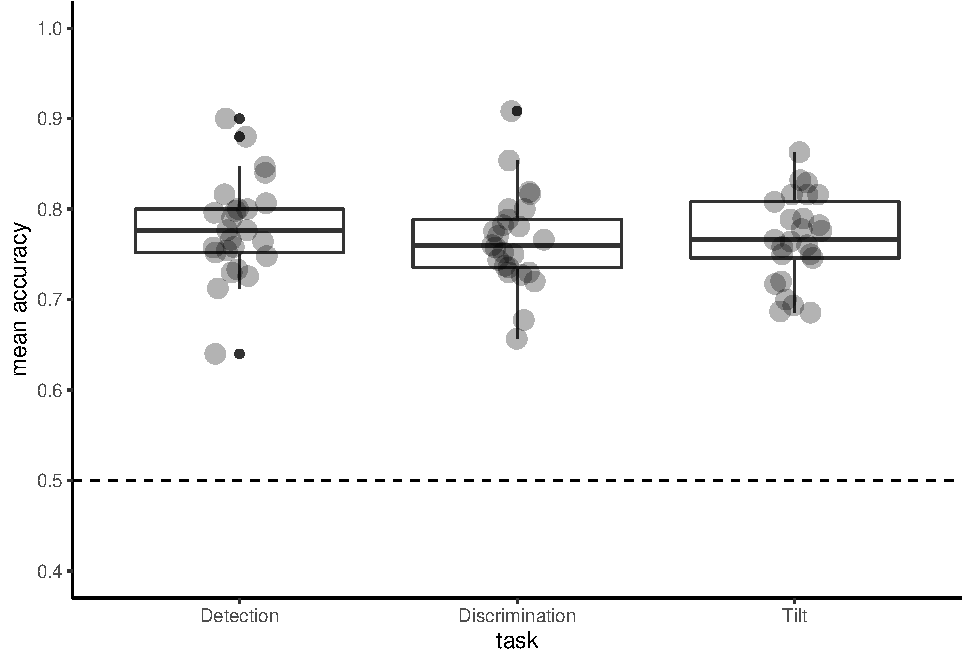
\includegraphics{Chudi-Thesis_files/figure-latex/accuracy_figure-1.pdf}
\caption{\label{fig:accuracy} Mean accuracy across three tasks}
\end{figure}

~

\hypertarget{confidence-distributions}{%
\subsection{4.2.Confidence
distributions}\label{confidence-distributions}}

Within detection, a significant difference in mean confidence was
observed between Yes (target present) and NO (target absent) responses
(see Fig.4 above) (t=-3.27, p = \textless{} 0.001) , such that
participants are more confident in their Yes responses than NO response
and a statistical significance was also observed in the tilt recognition
task between TILTED and Vertical response (t=-6.23, p = \textless{}
0.001; see Figure \ref{fig:confidence}).

\begin{figure}
\centering
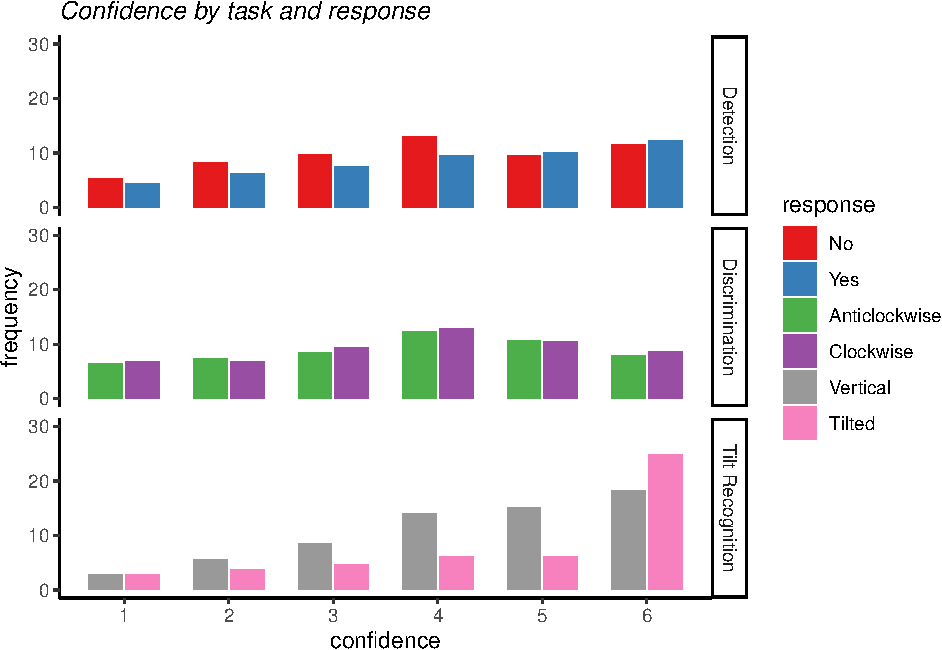
\includegraphics{Chudi-Thesis_files/figure-latex/unnamed-chunk-4-1.pdf}
\caption{\label{fig:confidence} Confidence distributions across three
tasks and responses. Error bars represent the standard error of the
mean.}
\end{figure}

~

~

\hypertarget{metacognitive-sensitivity}{%
\subsection{4.4.Metacognitive
sensitivity}\label{metacognitive-sensitivity}}

Metacognitive sensitivity, which is quantified as the area under Type 2
ROC curve (see \ref{fig:type2 ROC} ), is significantly higher for Yes
(0.72) than No (0.60) response. Similar pattern is observed in the tilt
recognition task, where the AUC is significantly higher for Tilted
(0.83) than Vertical (0.57) responses. This suggest that participants
confidence ratings are more diagnostic to accuracy in the judgments of a
target stimulus being pressent than being absent. Similarly, the correct
judgments of a stimulus being tilted is better reflected by partcipants'
confidence ratings than the correct judgments of a stimulus being
vertical.

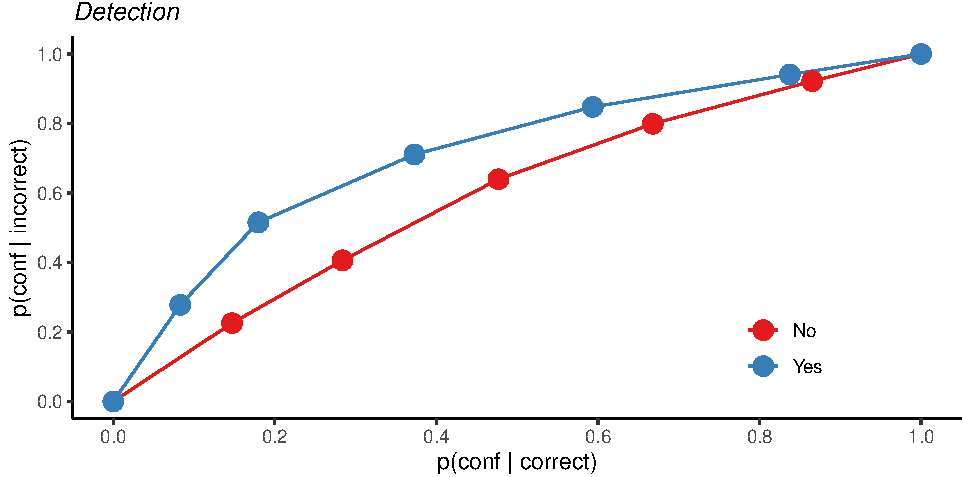
\includegraphics{Chudi-Thesis_files/figure-latex/fig-1.pdf}
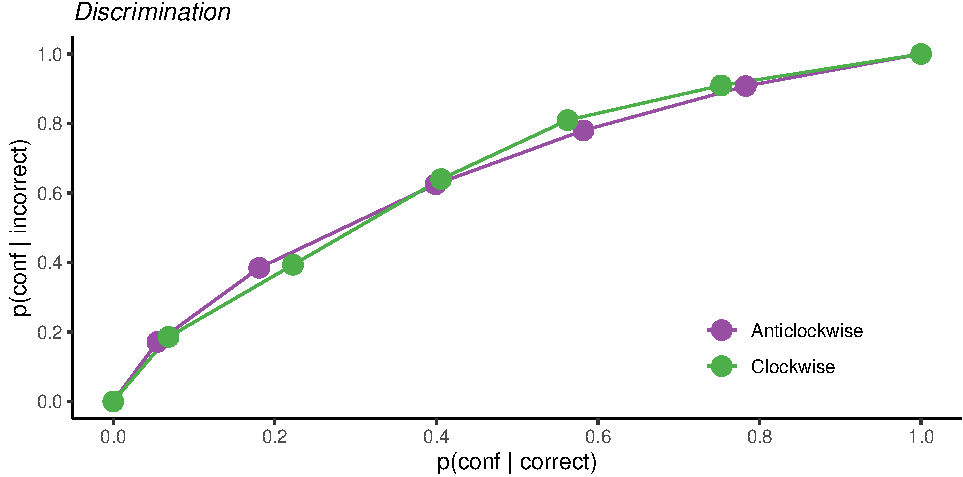
\includegraphics{Chudi-Thesis_files/figure-latex/fig-2.pdf}
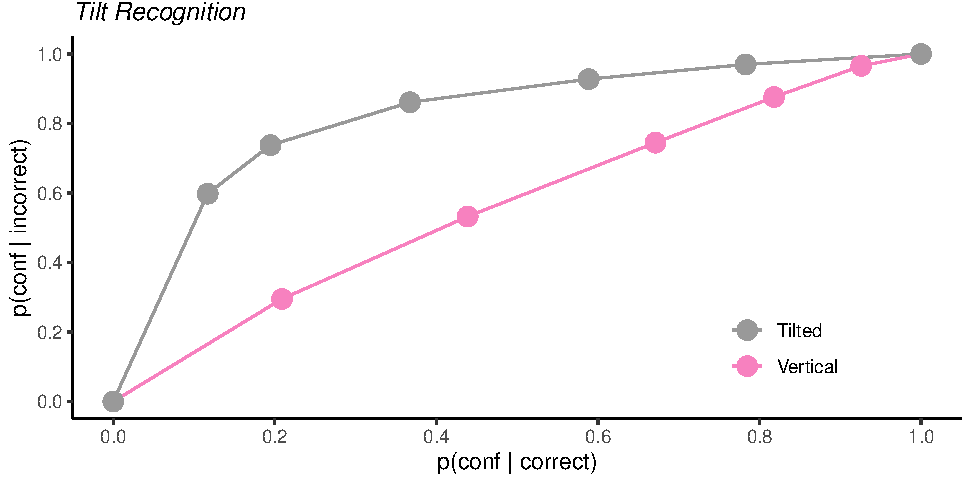
\includegraphics{Chudi-Thesis_files/figure-latex/fig-3.pdf}

~

~

\hypertarget{bold-signal-in-rois}{%
\subsection{4.5.BOLD signal in ROIs}\label{bold-signal-in-rois}}

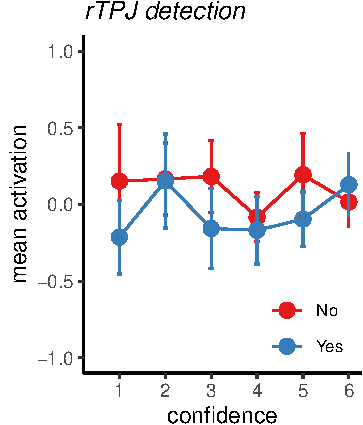
\includegraphics{Chudi-Thesis_files/figure-latex/unnamed-chunk-7-1.pdf}
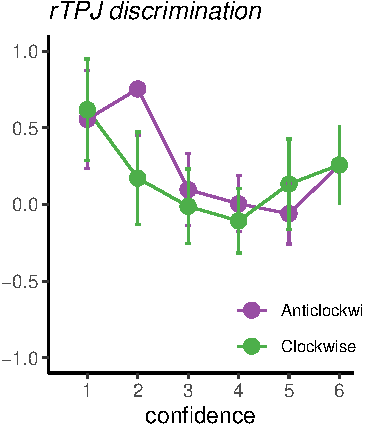
\includegraphics{Chudi-Thesis_files/figure-latex/unnamed-chunk-7-2.pdf}
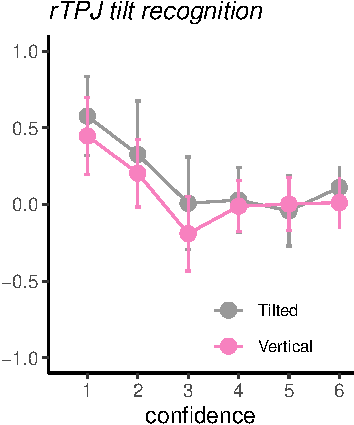
\includegraphics{Chudi-Thesis_files/figure-latex/unnamed-chunk-7-3.pdf}
~

~

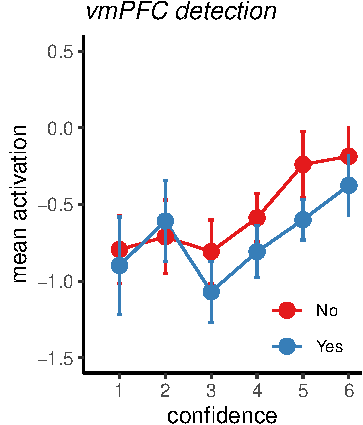
\includegraphics{Chudi-Thesis_files/figure-latex/unnamed-chunk-8-1.pdf}
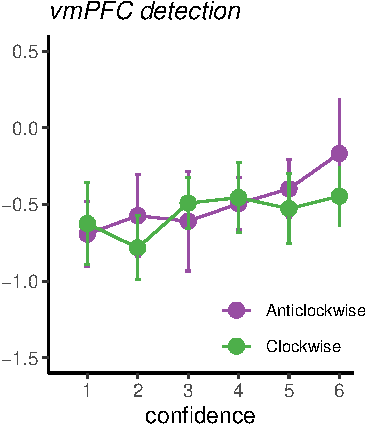
\includegraphics{Chudi-Thesis_files/figure-latex/unnamed-chunk-8-2.pdf}
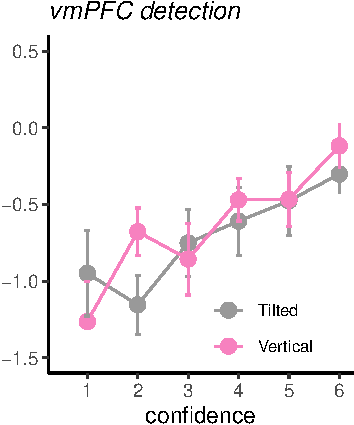
\includegraphics{Chudi-Thesis_files/figure-latex/unnamed-chunk-8-3.pdf}
~

~

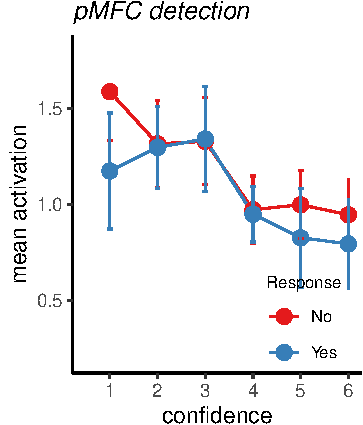
\includegraphics{Chudi-Thesis_files/figure-latex/unnamed-chunk-9-1.pdf}
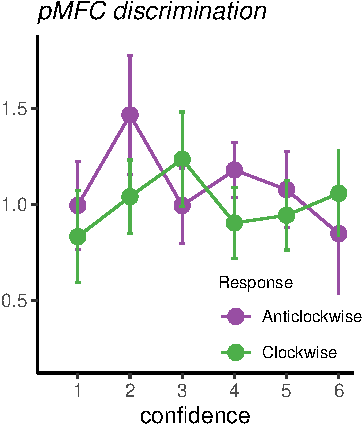
\includegraphics{Chudi-Thesis_files/figure-latex/unnamed-chunk-9-2.pdf}
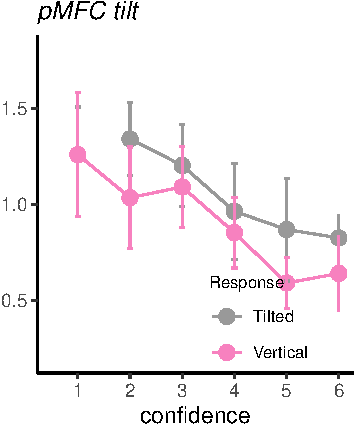
\includegraphics{Chudi-Thesis_files/figure-latex/unnamed-chunk-9-3.pdf}
~

~

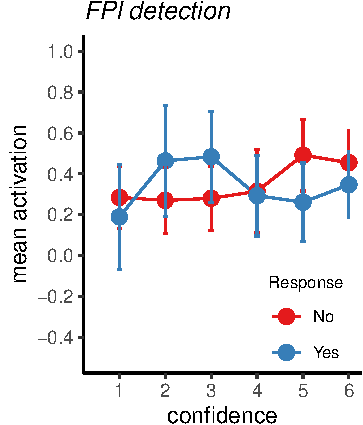
\includegraphics{Chudi-Thesis_files/figure-latex/unnamed-chunk-10-1.pdf}
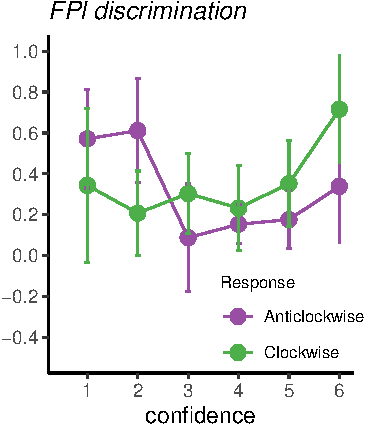
\includegraphics{Chudi-Thesis_files/figure-latex/unnamed-chunk-10-2.pdf}
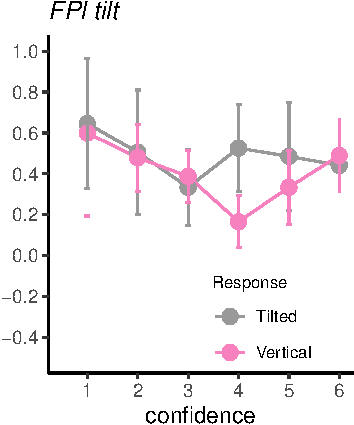
\includegraphics{Chudi-Thesis_files/figure-latex/unnamed-chunk-10-3.pdf}
~

~

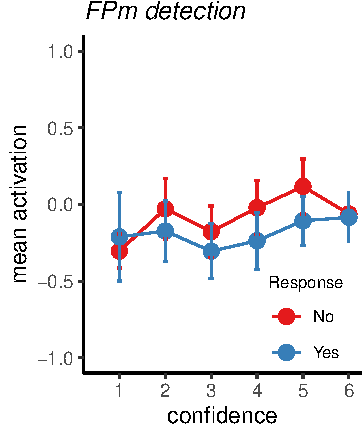
\includegraphics{Chudi-Thesis_files/figure-latex/unnamed-chunk-11-1.pdf}
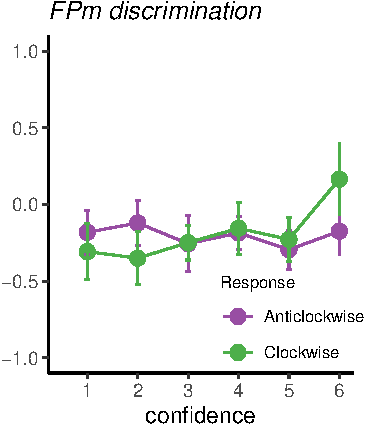
\includegraphics{Chudi-Thesis_files/figure-latex/unnamed-chunk-11-2.pdf}
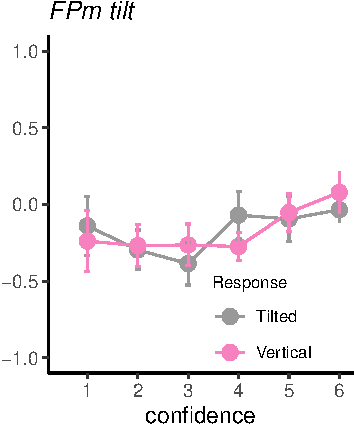
\includegraphics{Chudi-Thesis_files/figure-latex/unnamed-chunk-11-3.pdf}

\hypertarget{effect-of-confidence-on-bold-signal-in-rois}{%
\subsection{Effect of confidence on BOLD signal in
ROIs}\label{effect-of-confidence-on-bold-signal-in-rois}}

From our data, negative linear confidence-related effects were observed
in right Temporoparietal Junction (rTPJ) (\(\beta\)=-0.06, p=0.019),
Posterior Medial Frontal Cortex (pMFC)(\(\beta\)=-0.10, p=\textless{}
0.001), as well as polsitive linear correlation between confidence and
BOLD signals in Ventromedial Prefrontal Cortex (vmPFC)(\(\beta\)=0.12,
p=\textless{} 0.001), Medial Frontopolar Cortex (FPm)(\(\beta\)=0.04,
p=0.007).

To investigate whether linear effects of confidence on BOLD signal were
influenced by the type of task (Detection vs.~Discrimination vs.~Tilt
recognition) and/or reponse (Yes vs.~NO; Clockwise vs.~Anticlockwise;
Vertical vs.~Tilted), linear models with interactions were tested. The
effects of confidence failed to show a significant difference between
three tasks in all ROIs (all p values \textgreater{} 0.23). No
sognificant effect was observed between Yes and No response in detection
(all p values \textgreater{} 0.11), between Clockwise and Anticlockwise
responses in discrimination (all p values \textgreater{} 0.33) or
between Vertical and Tilted responses in tilt recognition (all p values
\textgreater{} 0.14).

~

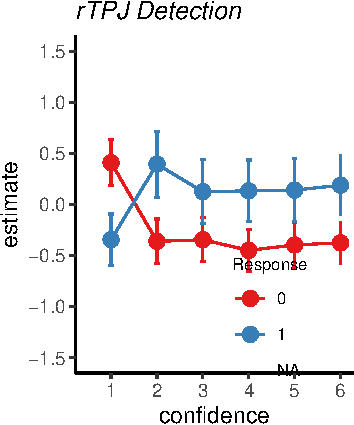
\includegraphics{Chudi-Thesis_files/figure-latex/mixed_effects-1.pdf}
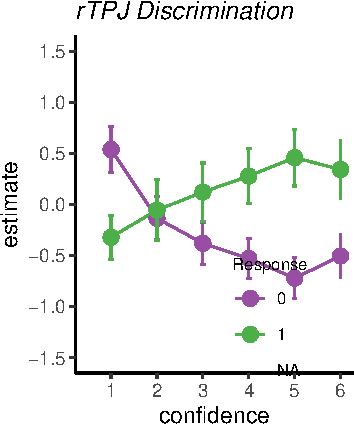
\includegraphics{Chudi-Thesis_files/figure-latex/mixed_effects-2.pdf}
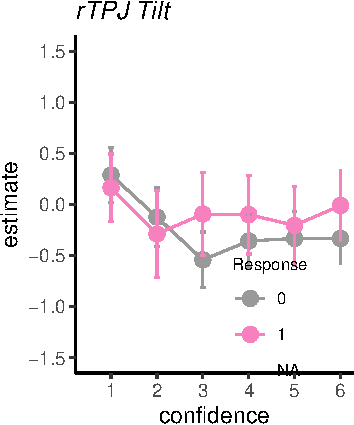
\includegraphics{Chudi-Thesis_files/figure-latex/mixed_effects-3.pdf}
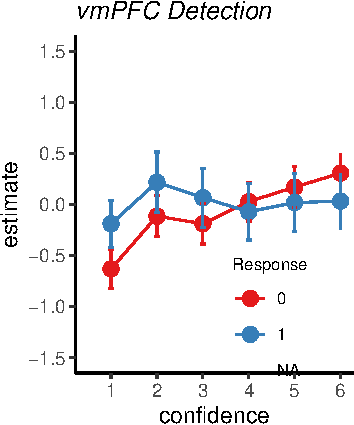
\includegraphics{Chudi-Thesis_files/figure-latex/mixed_effects-4.pdf}
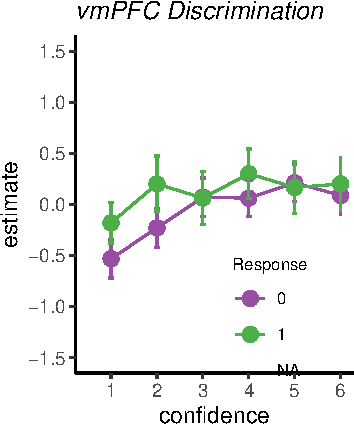
\includegraphics{Chudi-Thesis_files/figure-latex/mixed_effects-5.pdf}
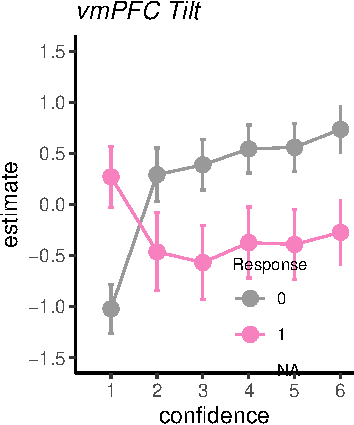
\includegraphics{Chudi-Thesis_files/figure-latex/mixed_effects-6.pdf}
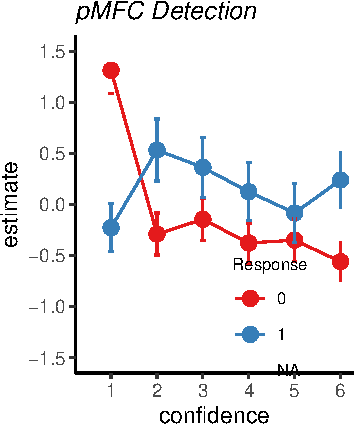
\includegraphics{Chudi-Thesis_files/figure-latex/mixed_effects-7.pdf}
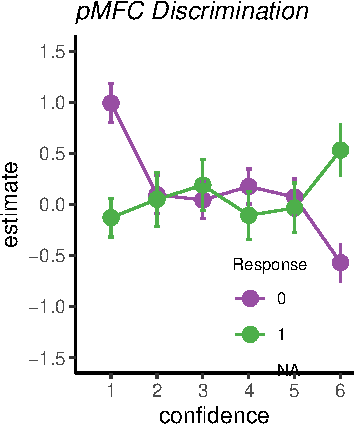
\includegraphics{Chudi-Thesis_files/figure-latex/mixed_effects-8.pdf}
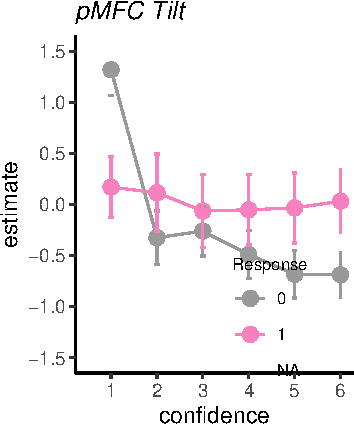
\includegraphics{Chudi-Thesis_files/figure-latex/mixed_effects-9.pdf}
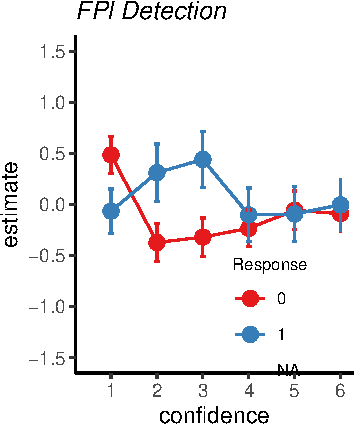
\includegraphics{Chudi-Thesis_files/figure-latex/mixed_effects-10.pdf}
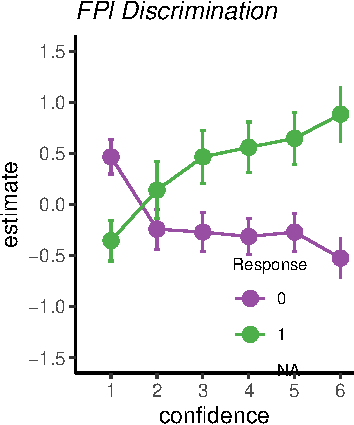
\includegraphics{Chudi-Thesis_files/figure-latex/mixed_effects-11.pdf}
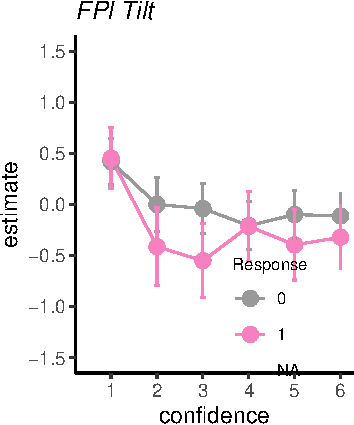
\includegraphics{Chudi-Thesis_files/figure-latex/mixed_effects-12.pdf}
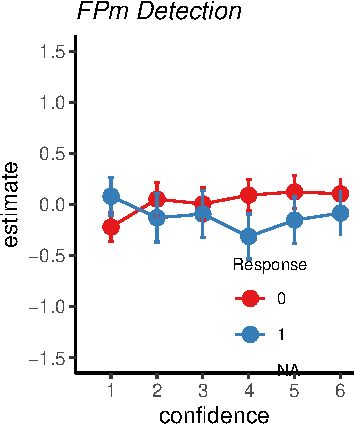
\includegraphics{Chudi-Thesis_files/figure-latex/mixed_effects-13.pdf}
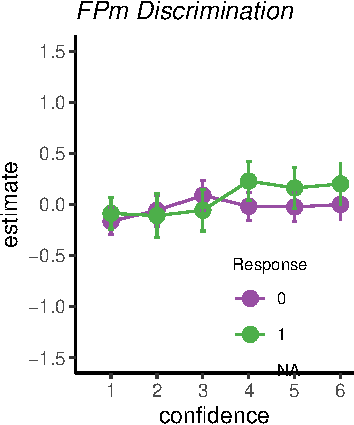
\includegraphics{Chudi-Thesis_files/figure-latex/mixed_effects-14.pdf}
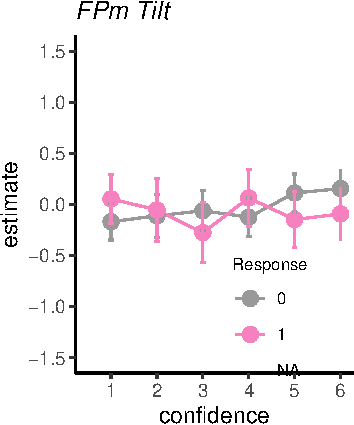
\includegraphics{Chudi-Thesis_files/figure-latex/mixed_effects-15.pdf} ~

\hypertarget{reference}{%
\subsection*{Reference}\label{reference}}
\addcontentsline{toc}{subsection}{Reference}

\hypertarget{refs}{}
\leavevmode\hypertarget{ref-adler2018pcb}{}%
Adler, William T., and Wei Ji Ma. 2018. ``Comparing Bayesian and
Non-Bayesian Accounts of Human Confidence Reports.'' \emph{PLoS
Computational Biology} 14 (11): e1006572.
\url{https://doi.org/10.1371/journal.pcbi.1006572}.

\leavevmode\hypertarget{ref-arielezylberberg2012fin}{}%
Ariel Ezylberberg, Ariel Ezylberberg, Ariel Ezylberberg, Pablo
Ebarttfeld, and Mariano Esigman. 2012. ``The Construction of Confidence
in a Perceptual Decision.'' \emph{Frontiers in Integrative Neuroscience}
6. Frontiers Media SA: 79.
\url{https://doi.org/10.3389/fnint.2012.00079}.

\leavevmode\hypertarget{ref-denison2018pnasusa}{}%
Denison, Rachel N., William T. Adler, Marisa Carrasco, and Wei Ji Ma.
2018. ``Humans Incorporate Attention-Dependent Uncertainty into
Perceptual Decisions and Confidence.'' \emph{Proceedings of the National
Academy of Sciences of the United States of America} 115 (43): 11090--5.
\url{https://doi.org/10.1073/pnas.1717720115}.

\leavevmode\hypertarget{ref-fleming2012ptrsb}{}%
Fleming, Stephen M., and Raymond J. Dolan. 2012. ``The Neural Basis of
Metacognitive Ability.'' \emph{Philosophical Transactions of the Royal
Society B} 367 (1594). The Royal Society: 1338--49.
\url{https://doi.org/10.1098/rstb.2011.0417}.

\leavevmode\hypertarget{ref-fleming_relating_2010}{}%
Fleming, Stephen M., Rimona S. Weil, Zoltan Nagy, Raymond J. Dolan, and
Geraint Rees. 2010. ``Relating Introspective Accuracy to Individual
Differences in Brain Structure.'' \emph{Science (New York, N.Y.)} 329
(5998): 1541--3. \url{https://doi.org/10.1126/science.1191883}.

\leavevmode\hypertarget{ref-grill-spector2005ps}{}%
Grill-Spector, Kalanit, and Nancy Kanwisher. 2005. ``Visual Recognition:
As Soon as You Know It Is There, You Know What It Is.''
\emph{Psychological Science} 16 (2). Blackwell Publishing: 152--60.

\leavevmode\hypertarget{ref-grimaldi2015nbr}{}%
Grimaldi, Piercesare, Hakwan Lau, and Michele A. Basso. 2015. ``There
Are Things That We Know That We Know, and There Are Things That We Do
Not Know We Do Not Know: Confidence in Decision-Making.''
\emph{Neuroscience and Biobehavioral Reviews} 55: 88--97.
\url{https://doi.org/10.1016/j.neubiorev.2015.04.006}.

\leavevmode\hypertarget{ref-kanai2010cc}{}%
Kanai, Ryota, Vincent Walsh, and Chia-Huei Tseng. 2010. ``Subjective
Discriminability of Invisibility: A Framework for Distinguishing
Perceptual and Attentional Failures of Awareness.'' \emph{Consciousness
and Cognition} 19 (4). Elsevier Inc: 1045--57.
\url{https://doi.org/10.1016/j.concog.2010.06.003}.

\leavevmode\hypertarget{ref-mack2010jephpp}{}%
Mack, Michael L., and Thomas J. Palmeri. 2010. ``Decoupling Object
Detection and Categorization.'' \emph{Journal of Experimental
Psychology: Human Perception and Performance} 36 (5). American
Psychological Association: 1067--79.
\url{https://doi.org/10.1037/a0020254}.

\leavevmode\hypertarget{ref-mazor2020e}{}%
Mazor, Matan, Karl J Friston, and Stephen M Fleming. 2020. ``Distinct
Neural Contributions to Metacognition for Detecting, but Not
Discriminating Visual Stimuli.'' Edited by Thorsten Kahnt, Joshua I
Gold, and Michael Graziano. \emph{eLife} 9 (April). eLife Sciences
Publications, Ltd: e53900. \url{https://doi.org/10.7554/eLife.53900}.

\leavevmode\hypertarget{ref-meuwese2014app}{}%
Meuwese, Julia D. I., Anouk M. Van Loon, Victor A. F. Lamme, and
Johannes J. Fahrenfort. 2014. ``The Subjective Experience of Object
Recognition: Comparing Metacognition for Object Detection and Object
Categorization.'' \emph{Attention, Perception \& Psychophysics} 76 (4):
1057--68. \url{https://doi.org/10.3758/s13414-014-0643-1}.

\leavevmode\hypertarget{ref-wickens2002}{}%
Wickens, Thomas D. 2002. \emph{Elementary Signal Detection Theory /
Thomas D. Wickens.} Oxford Scholarship Online. Oxford: University Press.

\end{document}
